%\documentclass[times, 10pt,twocolumn]{article}
%\usepackage{latex8}
%\usepackage{times}
\documentclass[10pt, conference, compsocconf]{IEEEtran}

\usepackage{amssymb,amsthm,amscd,bm}
\usepackage{graphicx}

\usepackage[tight,footnotesize]{subfigure}

\usepackage{url}

\usepackage{listings}
\lstset{language=C++, basicstyle=\normalsize}

\usepackage{mdwlist}

\makeatletter
\let\labelindent\@undefined
\makeatother
\usepackage{enumitem}

% take the % away on next line to produce the final camera-ready version
%\pagestyle{empty}

%\newcommand{\compact}{\setlength{\itemsep}{-\parsep}}
%\newcommand{\skipspace}{\vspace{-2mm}}
%\newcommand{\skipsectionspace}{\vspace{-3.5mm}}
\newcommand{\compact}{}
\newcommand{\skipspace}{}
\newcommand{\skipsectionspace}{}

\newcommand{\nC}{\mathbb{C}}

%\setlength{\intextsep}{0mm}
%\setlength{\floatsep}{0mm}
%\setlength{\textfloatsep}{3mm}
%\setlength{\dblfloatsep}{0mm}
%\setlength{\dbltextfloatsep}{0mm}
%\setlength{\abovecaptionskip}{0mm}
%\setlength{\belowcaptionskip}{0mm}


\begin{document}

\title{SmartDec: Approaching C++ Decompilation}

\author{\IEEEauthorblockN{Alexander Fokin\IEEEauthorrefmark{1},
Egor Derevenetc\IEEEauthorrefmark{2},
Alexander Chernov\IEEEauthorrefmark{3} and 
Katerina Troshina\IEEEauthorrefmark{4}}
\IEEEauthorblockA{\IEEEauthorrefmark{1}\IEEEauthorrefmark{3}Computational Math. and Cybernetics Dept., Moscow State University, Moscow, Russia\\ 
Email: \{apfokin, blackav\}@gmail.com}
\IEEEauthorblockA{\IEEEauthorrefmark{2}High Performance Computing Department, Fraunhofer ITWM, Kaiserslautern, Germany\\
Email: egor.derevenetc@itwm.fhg.de}
\IEEEauthorblockA{\IEEEauthorrefmark{4}Select LTD, Moscow, Russia\\
Email: katerina.dolgova@gmail.com\\}
}

\if 0
\author{
A. Fokin\\
Computational Math. and Cybernetics Dept.\\
Moscow State University\\
Leninskie Gory, Moscow, Russia\\
apfokin@gmail.com
\and
E. Derevenetc\\
High Performance Computing Department\\
Fraunhofer ITWM\\
Fraunhofer-Platz 1, Kaiserslautern, Germany\\
egor.derevenetc@itwm.fhg.de\\
\and
K. Troshina\\
Select LTD\\
Moscow, Russia\\
katerina.dolgova@gmail.com
\and
A. Chernov\\
Computational Math. and Cybernetics Dept.\\
Moscow State University\\
Leninskie Gory, Moscow, Russia\\
blackav@gmail.com
}
\fi

\maketitle
%\thispagestyle{empty}

\begin{abstract}\skipsectionspace
Decompilation is a reconstruction of a program in a high-level
language from a program in a low-level language. 
Typical applications of decompilation are software security 
assessment, malware analysis, error correction and reverse 
engineering for interoperability.

Native code decompilation is traditionally considered in the 
context of the C programming language.
C++ presents new challenges for decompilation, since the rules
of translation from C++ to assembly language are far more
complex than those of C.
In addition, when decompiling a program that was originally written
in C++, reconstruction of C++ specific constructs is desired.

In this paper we discuss new methods that allow partial
recovery of C++ specific language constructs from a low-level
code provided that this code was obtained from a C++ compiler.
The challenges that arise when decompiling such code are described. 
These challenges include reconstruction of polymorphic classes, class 
hierarchies, member functions and exception handling constructs.
An approach to decompilation that is used to overcome these challenges 
is presented.

SmartDec, a native code to C++ decompiler that is being 
developed by the authors at Select LTD is presented.
It reconstructs expressions, function arguments, local and global variables,
integral and composite types, loops and compound conditional statements,
C++ class hierarchies and exception handling constructs.
An empirical study of the decompiler is provided.
\end{abstract}

\begin{IEEEkeywords}
C++, Decompilation, Reverse Engineering, Class Hierarchy Reconstruction, Exception Reconstruction
\end{IEEEkeywords}


\section{Introduction}\skipsectionspace
Today it is not uncommon for a software development company to use
third-party components that are provided without source code.
In such cases it is often desired to verify that these components 
do not include malicious code and have no security loopholes. 
It is also a common situation when some legacy software 
is used for years and no source code is available.
%and there are no means of obtaining it.
In such situation a need may arise to fix errors in this software, 
improve its performance, or adapt it to the changed requirements. 

%Decompilation is a process of translation of a low-level programs 
%into a form that has a higher level of abstraction. 

Such problems are addressed by reverse engineering. 
Software reverse engineering may involve decompilation~--- 
translation of machine code or bytecode obtained from a compiler 
back into the source code in the original high level language. 
In order for decompilation to be correct, this source code, when compiled, 
must produce an executable with the same behaviour as that of the 
original program. 
% XXX: A decompilation output
Decompilation output won't be textually equivalent to the original 
source code, and is likely to be less comprehensible to a human. 

Native code decompilation is usually considered in the context of
the C programming language. 
A lot of research has been done on decompilation of C programs and 
existing decompilation methods show good results for programs that 
were originally written in C. 
Several successful commercial tools for C decompilation exist, 
including Hex-Rays \cite{hexrays}, Boomerang \cite{boomerang} and REC \cite{rec}. 
However, generally they do not perform well for C++ programs. 

Nowadays a great deal of software is written in C++ utilizing modern 
coding practices and patterns.
% XXX: the present-day software x2
The use of complex class hierarchies and exception handling in present-day software
is becoming more and more common, even in performance-critical applications,
such as database management systems. 
For example, C++ exceptions are used for error reporting in the kernel of the 
MongoDB document-oriented database \cite{mongodb}.
As the C++ specific constructs play significant role in internal 
workings of present-day software, it is important to reconstruct them fully
during decompilation.
Besides, decompilation of C++ programs into C results in undesirable 
artifacts, such as 
%unreferenced functions and cryptic code 
%fragments instead of C++ exception handling blocks, or several 
unrelated compound types and unions instead of C++ inheritance hierarchy.

In this paper we discuss new methods that allow partial
recovery of the C++ specific language constructs from a low-level
code provided that this code was compiled by a C++ compiler.
Compared to the C programming language, C++ introduces several new concepts,
presenting new challenges for decompilation. 
%These challenged include reconstruction of:
%\skipspace\begin{itemize}\compact
%\item classes and class hierarchies;
%\item virtual and non-virtual member functions, constructors and destructors;
%\item calls to virtual functions;
%\item types of class members and their layout;
%\item types of variables that store pointers to polymorphic classes (i.e. classes that use virtual functions);
%\item exception raising and handling statements.
%\end{itemize}
These challenges include reconstruction of classes and class hierarchies,
virtual and non-virtual member functions, calls to virtual functions,
exception raising and handling statements.
We propose solutions to these challenges and describe how they were 
implemented in SmartDec, a C++ decompiler.

We considered C++ ABI
(application binary interface) of Microsoft Visual Studio
compiler on Windows platform and C++ ABI
of GNU C++ compiler on Linux. We use MSVC 10.0 and g++ 4.5.0
for empirical study, but SmartDec also works for
other versions of these compilers provided they use the same C++ ABI.

%EXE -> ASM -> C -> C++ -> Refactoring.

%Decomp задачи:
%1. Functions.
%2. CFG.
%3. Types.

The rest of this paper is organized as follows. 
Section \ref{sectionRelatedWork} discusses related work.
Challenges of C++ decompilation along with possible solutions are
described in Section \ref{sectionChallenges}.
In Section \ref{sectionArchitecture} SmartDec decompiler is 
presented and its internal workings are described.
Experimental results are discussed in Section \ref{sectionExperiments}.
Our conclusions and directions for future work are
presented in the last section.




\section{Related work}\label{sectionRelatedWork}\skipsectionspace
Currently there exists no decompiler that is capable of reconstructing C++ code. 
There is some support for C++ in the latest version of the
Rec Studio, which supports mangled names and honors class inheritance hierarchy \cite{rec}.

Skochinsky \cite{skochinsky06e, skochinsky06c} has given a detailed description
of RTTI (run-time type information) and exception handling structures used by MSVC,
along with implementation details of some of the C++ concepts,
such as constructors and destructors.
He has presented tools for reconstruction of polymorphic class hierarchies and
exception handling statements in the assembly code.
However, these tools are based on pattern matching and do not always provide correct
results and cannot be used with compilers other than MSVC.

Sabanal and Yason \cite{sabanal07} along with RTTI-based approach
to class hierarchy reconstruction
have proposed a technique based on the analysis of vtables (virtual function tables) and
constructors that can be applied even when RTTI structures are
not present in the assembly.
Constructors are identified by searching for \textbf{operator new}
calls followed by a function call.
Vtable analysis is used for polymorphic class identification.
Class relationship inference is done via analysis of constructors.
Authors have also presented several examples of successful class
hierarchy reconstruction.
However, several cases in which presented techniques may fail are
not considered.
These cases include \textbf{operator new} overloading,
constructor inlining and elimination of vtable references in
constructors due to optimizations.
The presented techniques also heavily rely on the use of
MSVC-specific \textbf{\_\_thiscall} calling convention.

In \cite{fokin10} authors have proposed a
method for automatic reconstruction of class hierarchies
that does not rely on RTTI and performs well in cases
when aggressive optimizations are used by the compiler.




\section{Challenges of C++ Decompilation}\label{sectionChallenges}\skipsectionspace
Compared to the C programming language, C++ introduces several new concepts, including:
\skipspace\begin{itemize}\compact
\item Polymorphic classes and class hierarchies.
\item Virtual and non-virtual member functions.
\item Exceptions and exception handling.
%\item Templates.
\end{itemize}

%Templates are compile-time constructs that may leave no trace in 
%the binary code after compilation. 
%This is why reconstruction of templates is not considered in this paper.

Existing decompilation methods show good results for programs that 
were originally written in C. 
However, when decompiling C++ programs, 
C++ exception handling blocks are decompiled as several 
unreferenced functions in place of \lstinline{catch} blocks,
virtual function calls are not recognized, and classes 
are not reconstructed.

For quality C++ decompilation, the following constructs must be recovered:
\skipspace\begin{itemize}\compact
\item Virtual functions,
\item Classes,
\item Class hierarchies, i.e. inheritance relations between classes,
\item Constructors and destructors,
\item Types of pointers to polymorphic classes,
\item Non-virtual member functions,
\item Layout and types of class members,
\item Calls to virtual functions,
\item Exception raising and handling statements.
\end{itemize}


\subsection{Virtual functions}\skipsectionspace
In C++, a virtual function is a function with behaviour that can be 
% wikipedia :)
overridden within an inheriting class by a function with the same signature \cite{cpp03}. 
Virtual functions are an important part of the implementation of 
polymorphism in C++.

The C++ standard \cite{cpp03} does not mandate exactly how the 
virtual function dispatch must be implemented. 
In GCC \cite{gccabi} and MSVC \cite{gray94} ABIs it is
implemented using vtables. Each vtable is an 
array of pointers to virtual functions, therefore the problem of 
identification of virtual functions for MSVC and GCC can be 
reduced to the problem of locating all vtables.

In SmartDec vtables are located by scanning the data segment of the 
low-level code and checking each location in it as it is described in \cite{fokin10}. 


\subsection{Classes and class hierarchies}\skipsectionspace
The first approach to class hierarchy reconstruction utilizes
run-time type information as it is described in \cite{fokin10, sabanal07, skochinsky06c}. 
%RTTI in C++ is used for implementation of
%\lstinline{dynamic_cast<>} and \lstinline{typeid} operators \cite{stroustrup97}.
For each polymorphic class, an RTTI structure that 
contains information about its parents is emitted by the compiler.
All classes and complete polymorphic class hierarchy 
can then be reconstructed by examining all RTTI structures.

In GCC and MSVC C++ ABIs, a pointer to the RTTI structure
of a class always precedes its vtable \cite{gccabi, gray94}.
Therefore, the problem of finding RTTI structures can be reduced
to the problem of locating vtables.

% defined in the ABI || determined by the ABI
Layout of RTTI structures is defined by the ABI that is used by the C++ compiler.
Once the layout is known, RTTI structures can be parsed, thus
giving a complete polymorphic class hierarchy exactly as it was in the source C++ program.
Since run-time type information structures contain mangled class names, 
class names can also be recovered.

However, RTTI is considered to be frequently misused
\cite{stroustrup93}, and some modern applications written
in C++ refrain from using it. 
The use of RTTI increases binary size, and this is why it is
frequently disabled in code-size critical applications for
embedded systems \cite{quiroz98, cpppftr03}. 
Some frameworks replace RTTI with hand-rolled solutions because
it imposes a runtime overhead or is not powerful enough for the 
framework's needs.
Examples of such frameworks are Qt \cite{qt} and LLVM \cite{llvm}.
RTTI can be disabled at compile 
time, and in this case the above described approach to class 
hierarchy reconstruction cannot be used.

In case RTTI structures are not present in the assembly, 
an approach based on the analysis of vtables,
constructors and destructors can be used for reconstruction of
polymorphic class hierarchies as it is described in \cite{fokin10}.

In SmartDec both approaches are implemented.

% TODO: so, what is new here?


\subsection{Constructors and destructors}\skipsectionspace
In SmartDec constructors and destructors are detected for polymorphic classes only. 
Constructors and destructors of non-polymorphic classes do not differ from
ordinary member functions, and therefore are difficult to detect reliably. 
This is one of the directions of future work.

\begin{figure}[tb!]
\begin{minipage}[b]{0.49\linewidth}
\centering
  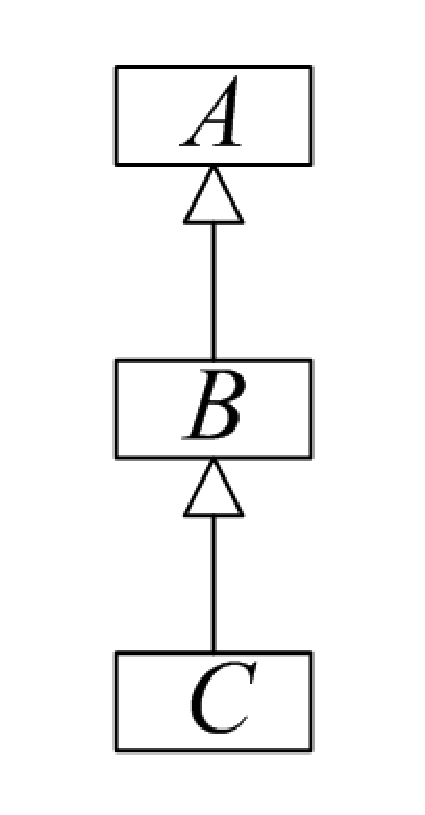
\includegraphics[height=3.0cm]{images/abc}
\caption{Example of a class hierarchy.}
\label{fig:abc}
\end{minipage}
%\hspace{0.1cm}
\begin{minipage}[b]{0.49\linewidth}
\centering
  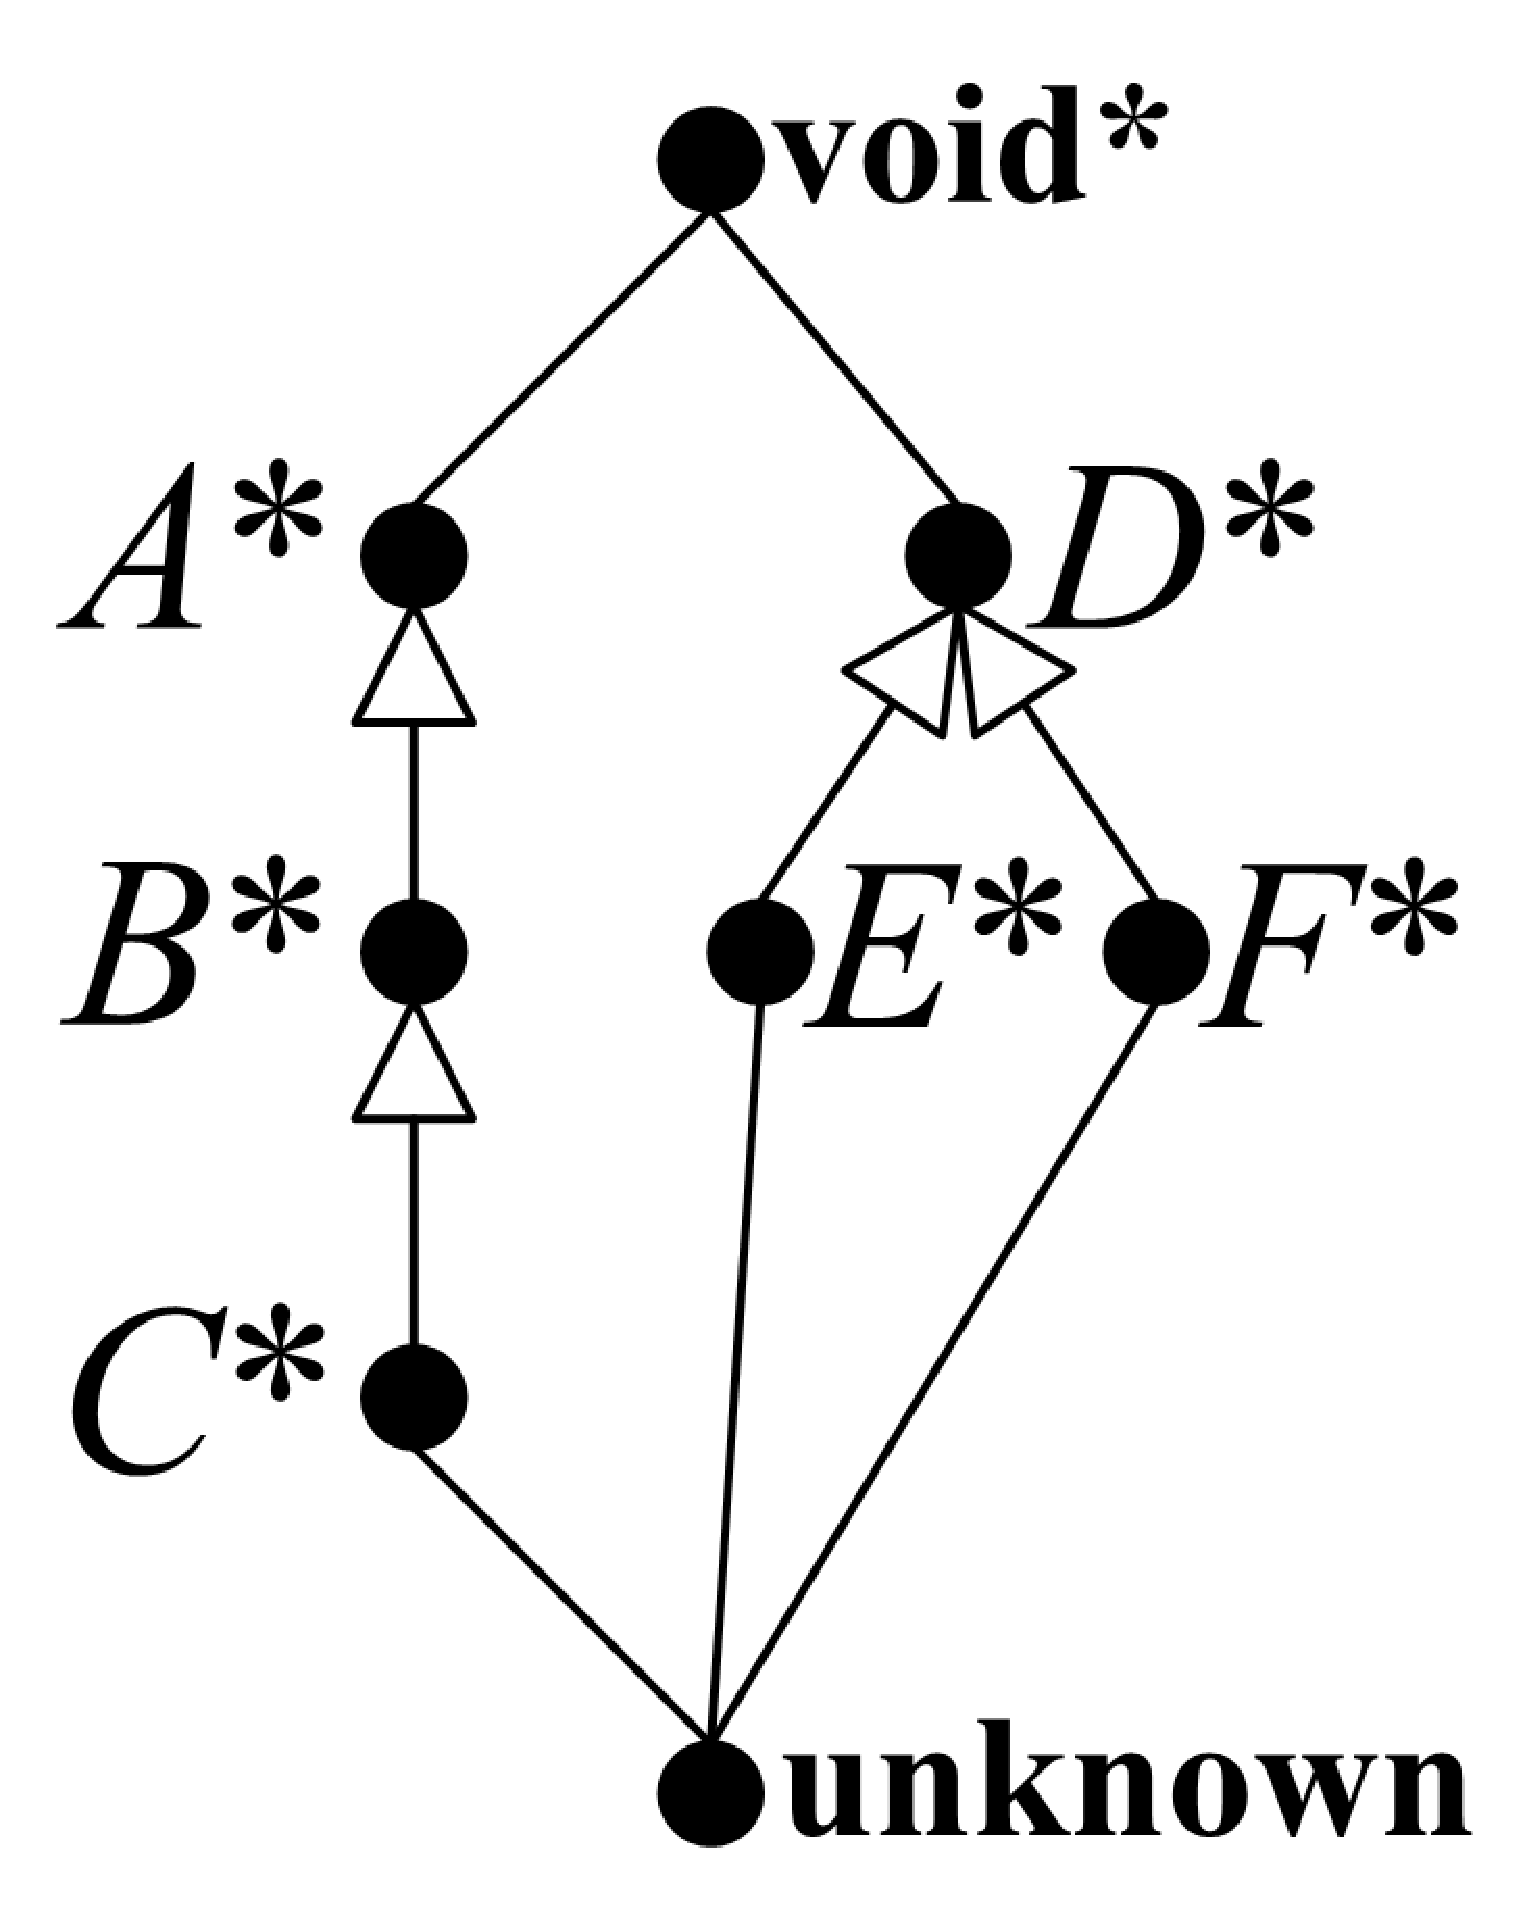
\includegraphics[width=3.0cm]{images/lattice}
%\vspace{-3mm}
\caption{Example of a type lattice.}
\label{fig:lattice}
\end{minipage}
\end{figure}

\begin{figure}[tb!]
\centering
  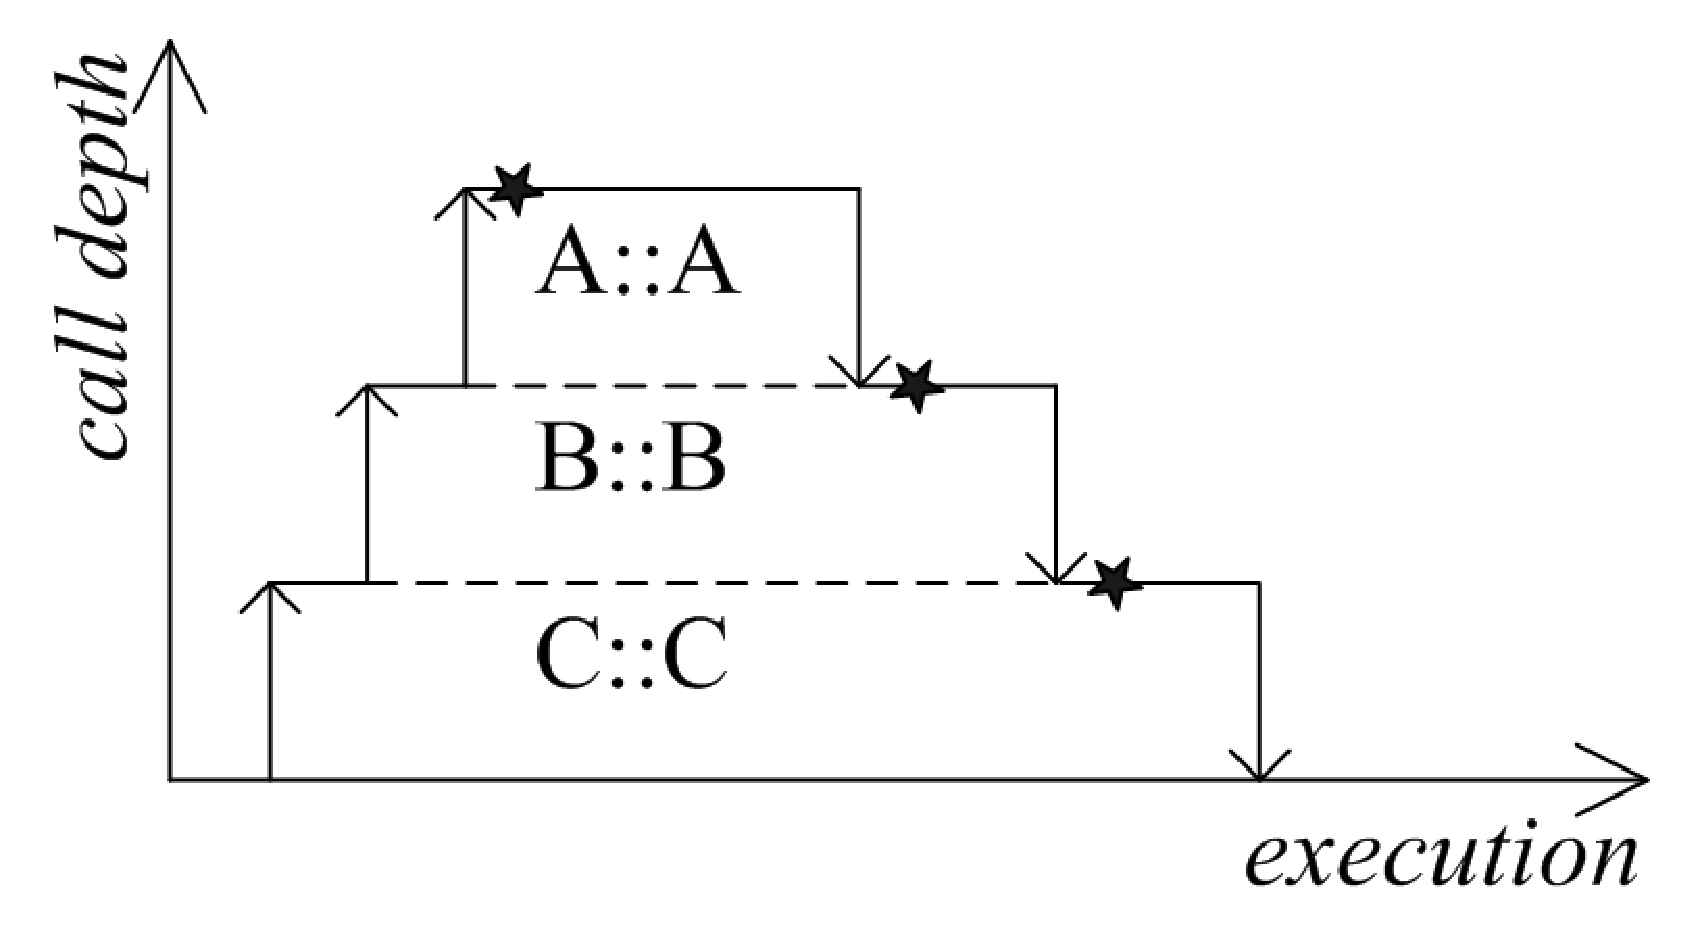
\includegraphics[width=6.0cm]{images/ctor}
%\vspace{-4mm}
\caption{Outline of constructor execution for class \lstinline{C} from Fig \ref{fig:abc}.
Initializations of vtable pointer field are marked with $\bigstar$.}
\label{fig:ctor}
\end{figure}

\begin{figure}[tb!]
\centering
  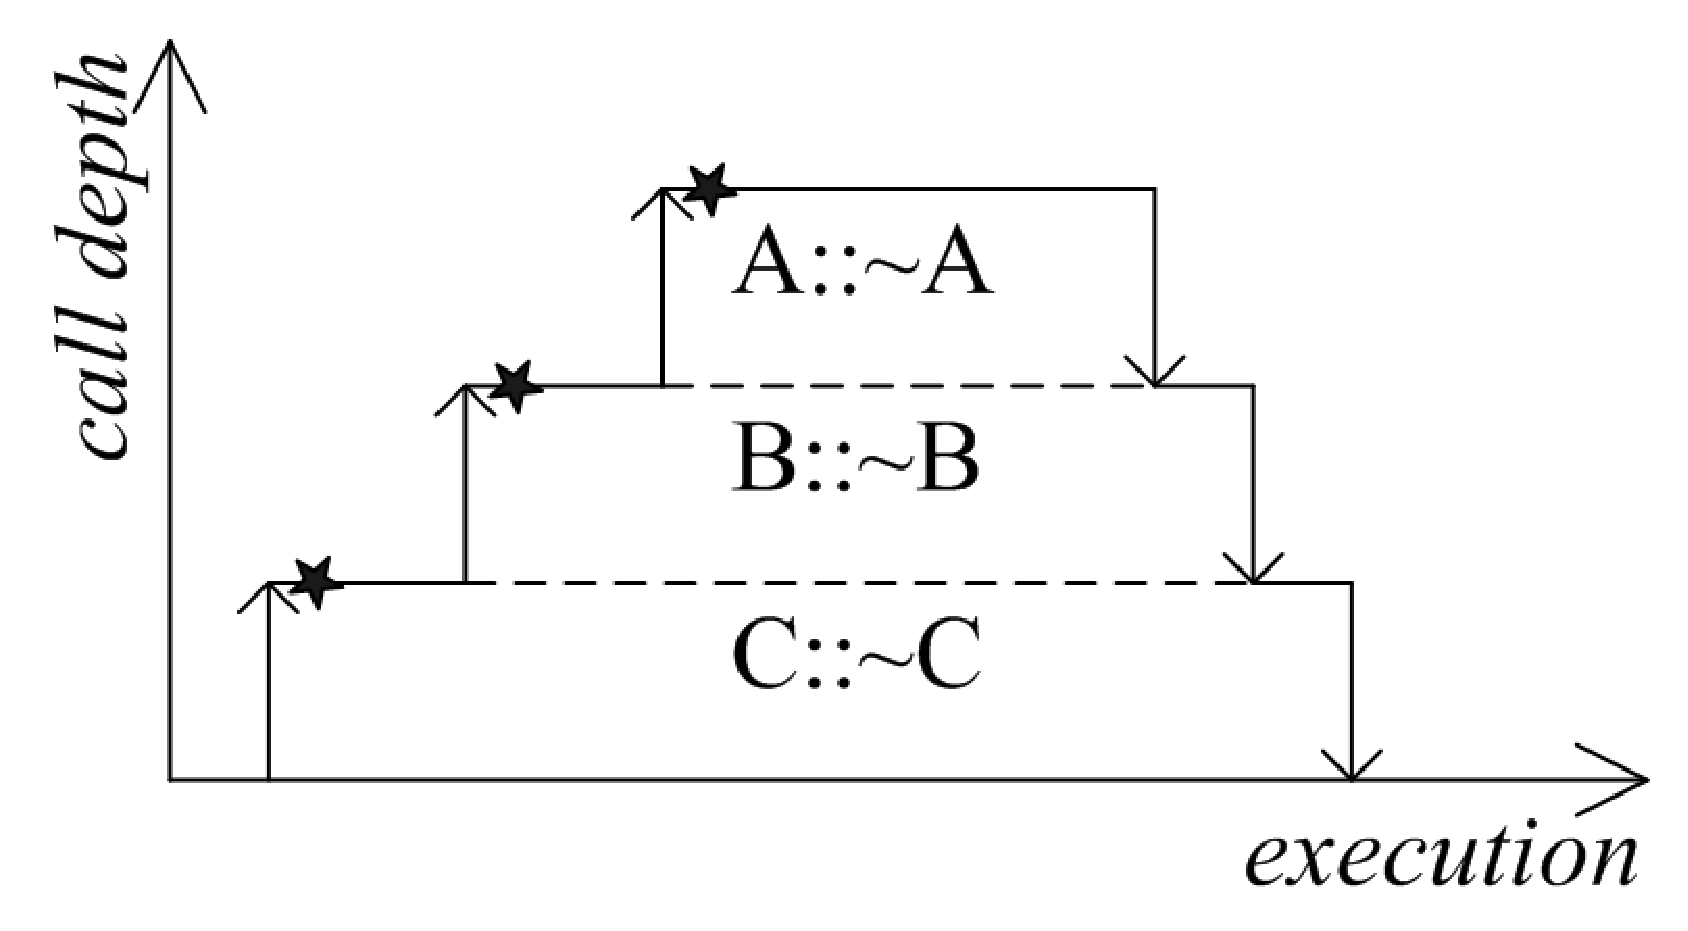
\includegraphics[width=6.0cm]{images/dtor}
%\vspace{-4mm}
\caption{Outline of destructor execution for class  \lstinline{C} from Fig \ref{fig:abc}.
Initializations of vtable pointer field are marked with $\bigstar$.}
\label{fig:dtor}
\end{figure}

Constructors and destructors are detected by checking the operations they perform
as it is described in \cite{fokin10}.
A constructor of a class performs the following sequence
of operations \cite{cpp03, gray94}:
\skipspace\begin{enumerate}\compact
\item calls constructors of direct base classes;
\item calls constructors of data members;
\item initializes vtable pointer field(s) and
      performs user-specified initialization code in the body
      of the constructor.
\end{enumerate}

Conversely, a destructor deinitializes the object
in the exact reverse order to how it was initialized:
\skipspace\begin{enumerate}\compact
\item initializes vtable pointer field(s) and
    performs user-specified destruction code in the body of the destructor;
\item calls destructors of data members;
\item calls destructors of direct bases.
\end{enumerate}

Interprocedural data flow analysis is used to detect consequent 
vtable pointer field initializations, thus locating constructors
and destructors. This approach also makes it possible to detect 
inlined constructors and destructors.

The order in which vtable pointer field initializations are performed
is determined by the inheritance order. 
Consider hierarchy in Fig.~\ref{fig:abc}.
Outlines of constructor and destructor execution for class \lstinline{C} 
are provided on Fig.~\ref{fig:ctor} and \ref{fig:dtor} correspondingly. 
As can be seen, in a call to constructor vtable
pointer field is overwritten in a ``base-to-derived'' order,
while in a call to destructor it is overwritten in a
``derived-to-base'' order.
Also in a call to constructor, vtable pointer field is initialized \textit{after} a
call to the constructor of the base class, while in a call to a destructor,
vtable pointer field is initialized \textit{before} a call to the destructor of
the base class. 
These heuristics are used to distinguish constructors from destructors.

%\begin{figure}[tb!]
%\centering
%  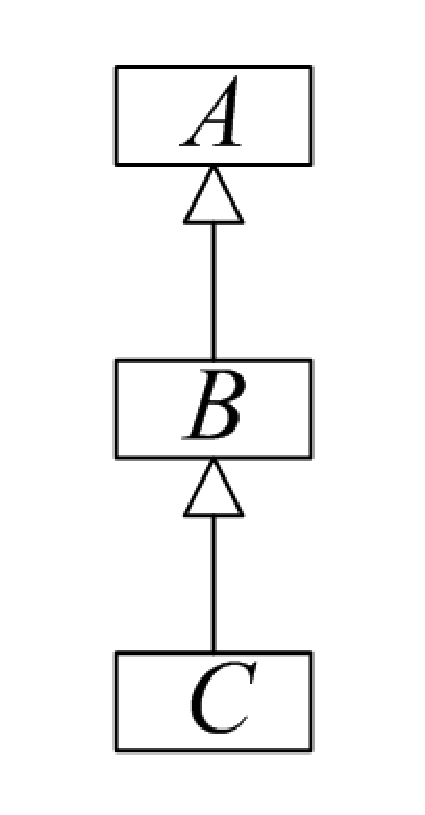
\includegraphics[height=3.0cm]{images/abc}
%\caption{Example of a class hierarchy.}
%\label{fig:abc}
%\end{figure}

\subsection{Class pointers}\skipsectionspace
Class pointers may appear in several different contexts.
In each of these contexts several different values may be assigned to a single class pointer:
\skipspace\begin{itemize}\compact
\item A variable or a composite type member may be assigned a value several times.
\item A function may be called from several different locations, 
  with pointers to different classes from the same hierarchy passed to it as parameters.
\item A function may have several exit points, and pointers to different
  classes may be returned at each of them.
\end{itemize}

A reconstructed type of a pointer must be compatible with types 
of all values assigned to it.
That is, it must either be a superclass of all of them, or a generic 
\lstinline{void*} pointer.
This can be achieved using a lattice model for pointer type 
reconstruction.
First, class hierarchy is recovered and a type lattice $(\nC, \rhd)$ is 
constructed, where $\nC$ is a set of pointer types that consists of:
\skipspace\begin{itemize}\compact
\item the pointers to all recovered class types;
\item \lstinline{void*} pointer;
\item special \textbf{unknown} pointer type.
\end{itemize}

The partial order $\rhd$ is defined by the inheritance relation on a set of
classes with addition of the following elements:
\skipspace\begin{itemize}\compact
\item For all $A \in \nC$ that are the roots of inheritance hierarchy, $A \rhd$~\lstinline{void*}.
\item For all $A \in \nC$ that are the leafs of inheritance hierarchy, \textbf{unknown}~$\rhd A$.
\end{itemize}

%\begin{figure}[t!]
%\centering
%  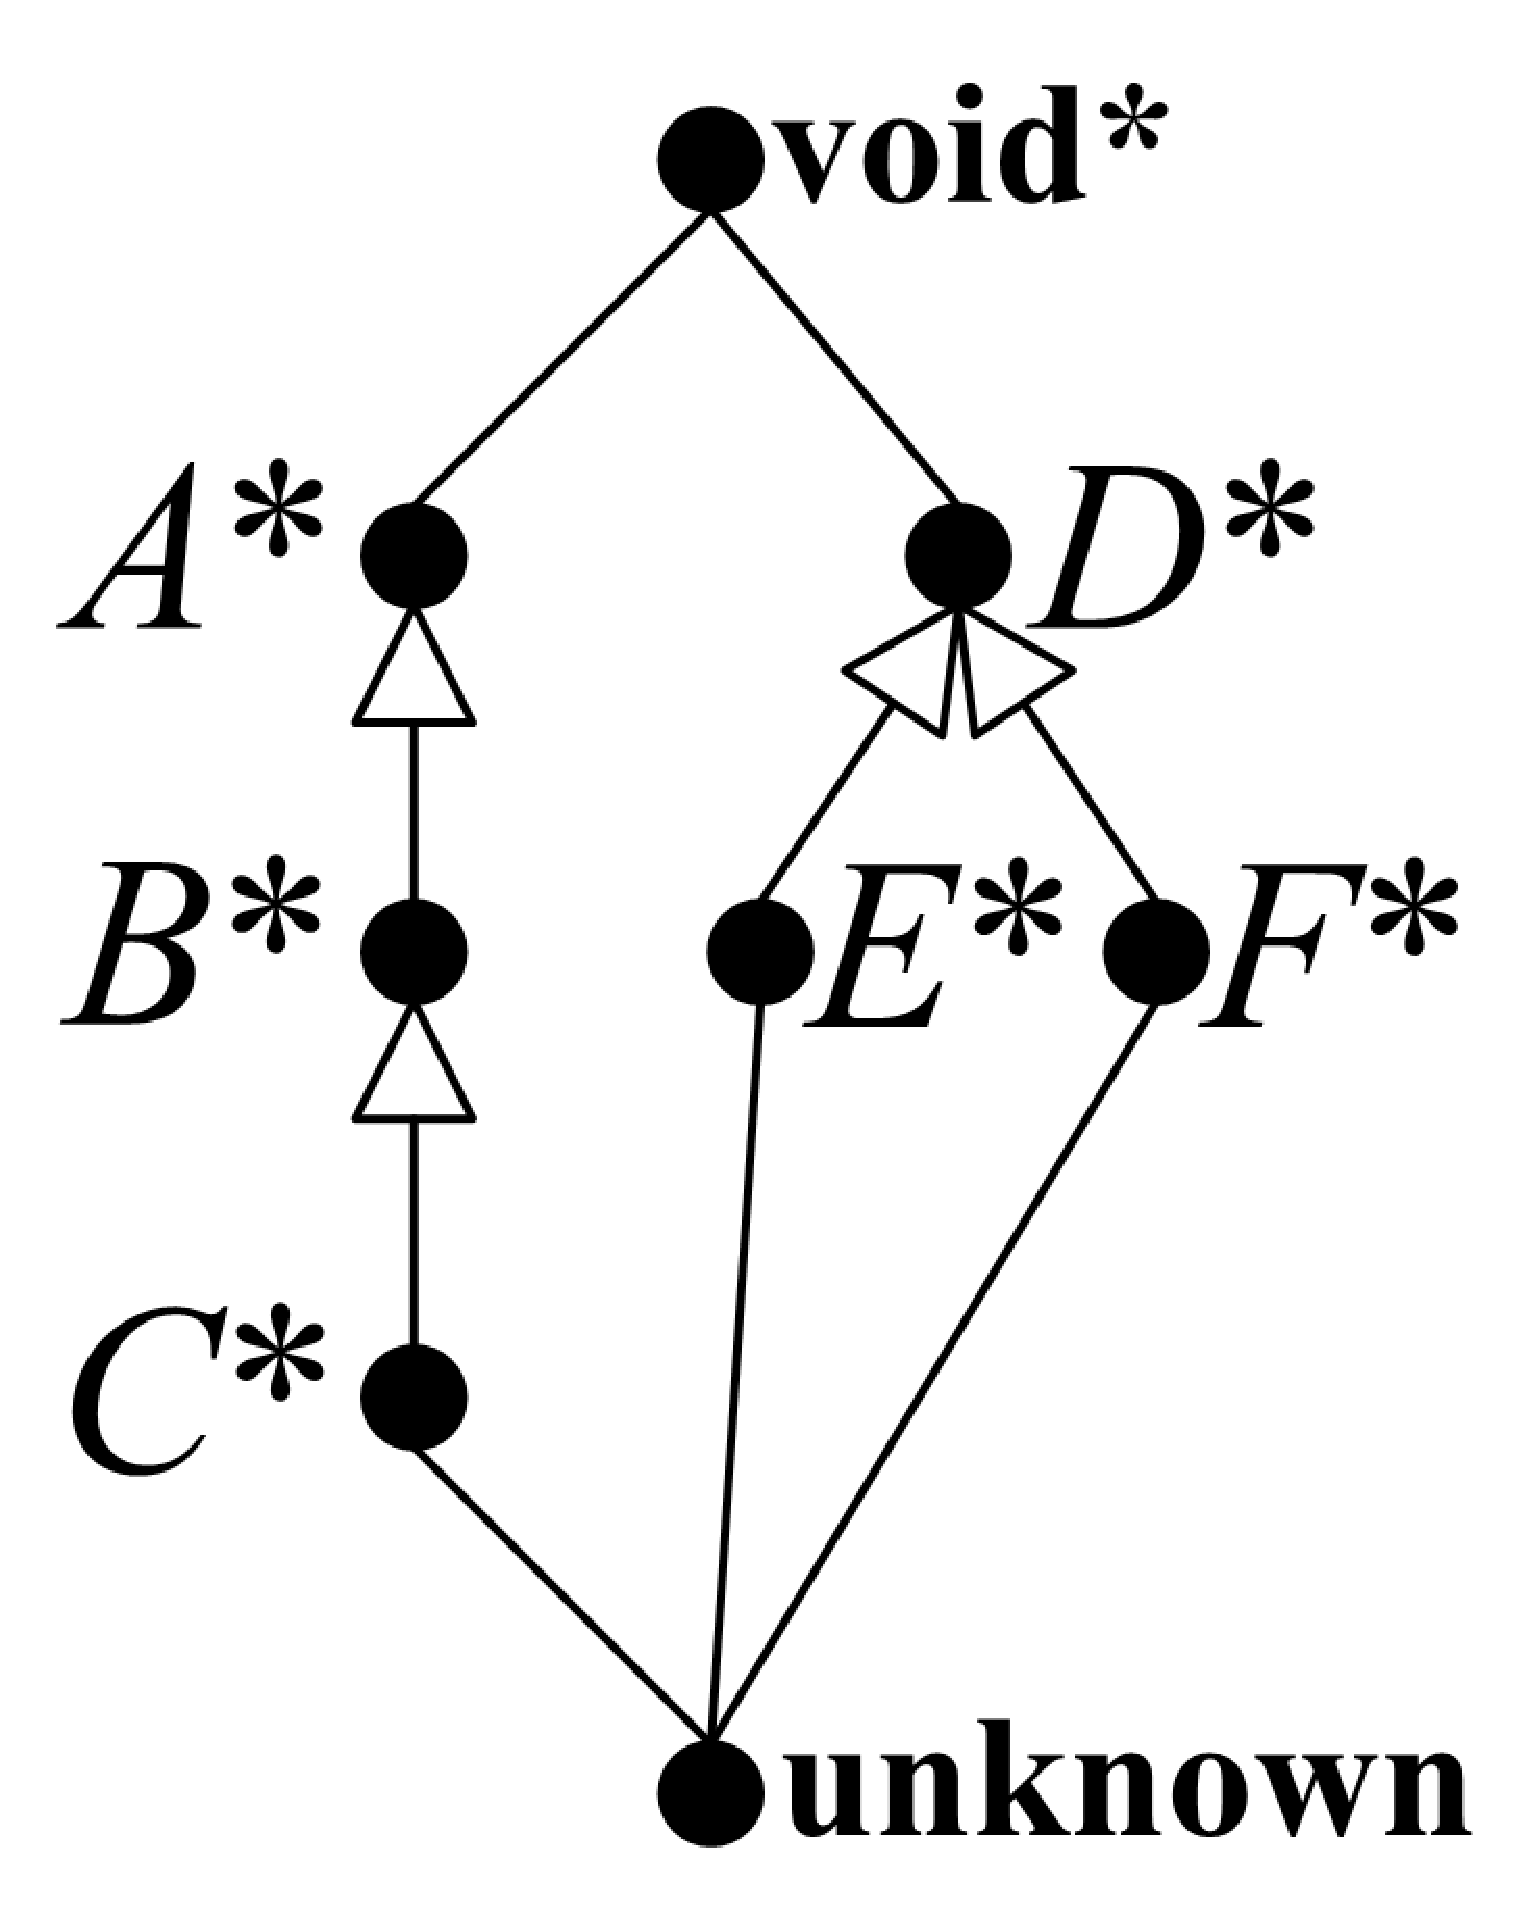
\includegraphics[width=3.0cm]{images/lattice}
%\caption{Example of a type lattice.}
%\label{fig:lattice}
%\end{figure}

Example of a Hasse diagram for type lattice is presented on Fig.~\ref{fig:lattice}. 
For convenience, inheritance relations are depicted on the diagram in UML notation.

Initially, a type of a pointer is initialized to \textbf{unknown}. 
On each assignment, its type is set to the least common ancestor of its 
current type and the type of the value that is assigned to it.

Constructors that were identified on the previous step are known to return pointers
of specific class types. 
This type information is then iteratively propagated through the assignments and function 
calls using the above described model for type resolution.

% TODO: what if downcasts occur in a program?
% Well... there are problems actually. If there is a static downcast followed by a 
% virtual function call, then how do we resolve it?


\subsection{Member functions}\skipsectionspace
When reconstructing non-virtual functions, it is often desired to determine if a 
function at hand is a member function and to find the class that it belongs to.
In GCC ABI member functions are indistinguishable from free-standing functions with 
\lstinline{this} pointer passed as the first parameter. 
With such ABI reliable reconstruction of member functions is not generally 
possible and must be performed manually. 
MSVC by default uses \lstinline{__thiscall} calling convention for 
member functions, which passes \lstinline{this} pointer in \verb|ECX| register. 
In this case member functions can be reliably distinguished.
The class that the member function belongs to is then determined by the
type of \lstinline{this} parameter.

% TODO: what about GCC? Manually?


\subsection{Composite types}\skipsectionspace
Type reconstruction algorithms~\cite{mycroft1999,wcre2008} typically assume 
that copies of the same pointer always reference values of the same type.
In C++ this assumption is usually broken because during program execution the same pointer 
may point to objects of different classes from the same hierarchy.
As a result, composite type reconstruction algorithm \cite{scam2010} merges information 
about the types of the base class fields and the fields of its subclasses.
Since different subclasses typically have fields of different types at the 
same offsets, such aggregation leads to type clashes and incorrect type reconstruction.

This problem is solved using reconstructed information about class pointers. 
All accesses to class fields (i.e. accesses to memory locations at constant
offsets from object pointer) are considered. For each access, the sum
of this constant offset and corresponding memory location's size is computed.
Maximum of computed sums for each class is taken as the underapproximation of
class's size.

The decompiler implements modified version of the type reconstruction
algorithm \cite{scam2010}, which avoids merging information about fields
lying outside the approximated object size, thus preventing type clashes.


\subsection{Virtual function calls}\skipsectionspace

For the reconstruction of virtual functions to be complete, calls to virtual functions
must also be reconstructed. 
Some compiler optimizations may result in virtual calls being
devirtualized and replaced by ordinary functions calls, or even inlined \cite{namolaru06, bacon96, porat96}.
When not devirtualized or inlined, a virtual function call is compiled into 
a sequence of assembly instructions that extracts a function pointer from
the vtable and performs an indirect call. 
An example of such a sequence produced by MSVC is presented in Fig.~\ref{fig:vcall}.

Virtual function calls are reconstructed after the types of the variables are recovered.
Once the type of the object pointer that is used for a virtual function call is known, 
a simple pattern matching approach is used to detect virtual function calls.
Each detected virtual function call may provide additional information about
parameter types of the corresponding virtual function. 
This is why once a virtual function call is detected, 
the type analysis is rerun for all of the affected virtual functions.

\begin{figure}[tb!]
\centering
{
\lstset{basicstyle=\scriptsize, language=[x86masm]Assembler}
\begin{lstlisting}
; The following code performs the call 
; object->function(20).
; Pointer to object is stored in esi.
; First, vtable pointer is loaded to eax
mov  eax, dword ptr [esi]
; Virtual function pointer is loaded to edx
mov  edx, dword ptr [eax+4] 
; Argument is passed on the stack
push 14h  
; `this` pointer is passed in ecx register
mov  ecx,esi
; Finally, virtual function is called
call edx  
\end{lstlisting}
%\vspace{-5mm}
}
\caption{Example of a virtual function call produced by MSVC.}
% TODO: alike for GCC?
\label{fig:vcall}
\end{figure}

\subsection{Exception handling}\skipsectionspace
%
% start with CFG
%
Exception handling is a C++ concept designed to handle the occurrence of exceptions, 
special conditions that change the normal flow of program execution. 
Exception handling is normally used for reporting and handling errors that 
occur during program execution in a uniform way.

%Matching of exception types and the types of \lstinline{catch} blocks is
%performed at runtime. This is why exception handling implementation
%requires not only support from the code generator, but also typically 
%involves additional support from the runtime system accompanying it.

The C++ standard defines the semantics of exception raising and handling,
but leaves its implementation up to compiler vendors. 
%Two implementation schemes are most common.
We have considered two implementation schemes.
In the first scheme, used by MSVC, the compiler generates code that continuously updates exception 
handling structures to reflect the current program state. 
A new element is added to the stack frame layout that
contains the information on exception handlers that are available
for the function associated with that frame.
If an exception is thrown, this element is used by the runtime support library
to locate and execute the appropriate exception handler \cite{kocchar02}.

The second scheme, used by GCC, employs a table-driven approach and introduces no 
runtime overhead if exceptions are not used. 
It involves the creation of statically allocated tables that
relate ranges of the program counter to the program state. 
When an exception is thrown,
the runtime system looks up the current value of the program counter in
these tables and determines which handlers are to be checked \cite{gccabi}.

Exception handling, while a high-level concept, involves low-level
manipulations that do not translate well into C. For example, non-trivial 
control flow of the exception handling cannot be implemented
in C without assembly. 
Many algorithms for control flow analysis \cite{muchnick97} do not take exception handling into account. % TODO: more cite
As a result, \lstinline{catch} blocks are isolated into separate functions. 
This is why proper reconstruction of
exception handling requires intervention on several decompilation stages 
and cannot be implemented as a post-processing step that would
fix the decompiled C code.

% TODO: is citing Muchnick OK?
In SmartDec, exception handling structures are located and parsed after 
construction of the control flow graph, and additional edges of a special kind are 
inserted into it. 
These edges connect \lstinline{catch} blocks with the functions they belong to, 
thus preventing them from being isolated into separate functions.
On the high-level program generation step this edge kind information is used to guide 
the reconstruction of actual \lstinline{catch} blocks.

Exception propagation involves the execution of destructors. As destructors for
non-polymorphic classes are frequently inlined, SmartDec is currently
unable to fully recognize and recover them. This is why destructor code
is currently output as comments and must be integrated into the program 
manually.

Due to the differences in exception handling implementations between compilers,
there is no universal way of reconstructing \lstinline{try} blocks and 
\lstinline{throw} statements. We describe how these constructs can be 
reconstructed for programs compiled with GCC.



\subsubsection{Exception handling in GCC}
GCC for x86 and x64 architectures by default uses Dwarf2 table-based unwinding mechanism.
In Dwarf2 each function is associated with a set of \textit{call sites}. 
Call sites are code sections that can potentially throw an exception, 
e.g. function calls or \lstinline{throw} statements. 
Each call site is associated with a \textit{landing pad}.
A landing pad is a code block that calls destructors and transfers 
execution to the corresponding \lstinline{catch} block. 
Example of a landing pad is presented on Fig. \ref{fig:lpad}.
Information about call sites and landing pads is statically allocated and is present in the low-level code. 
Details on the format of this information and on how exception
handling is performed using it is given in \cite{gccabi} and \cite{linuxspec}.

\begin{figure}[tb!]
\centering
{
\lstset{basicstyle=\scriptsize, language=[x86masm]Assembler}
\begin{lstlisting}
; Destructor calls skipped.
; Exception pointer is passed in eax.
mov [ebp - 24], eax
; Index in the type table is passed in edx.
mov [ebp - 28], edx
cmp [ebp - 28], 2
je catch_block_2
cmp [ebp - 28], 1
je catch_block_1
mov eax, [ebp - 24]
mov [esp], eax
call _Unwind_Resume
\end{lstlisting}
%\vspace{-5mm}
}
\caption{Example of a landing pad.}
\label{fig:lpad}
\end{figure}

%\textbf{.eh\_frame} section of the assembly contains information on stack frames
%that is needed for stack unwinding. Its format is described in \cite{linuxspec}.
%Frame descriptor for each function contains a pointer to the
%Language Specific Data Area (LSDA) containing exception handling information (see Fig.~\ref{fig:gcce}).
%LSDAs are stored in \textbf{.gcc\_except\_table} section.

\begin{figure}[tb!]
\centering
  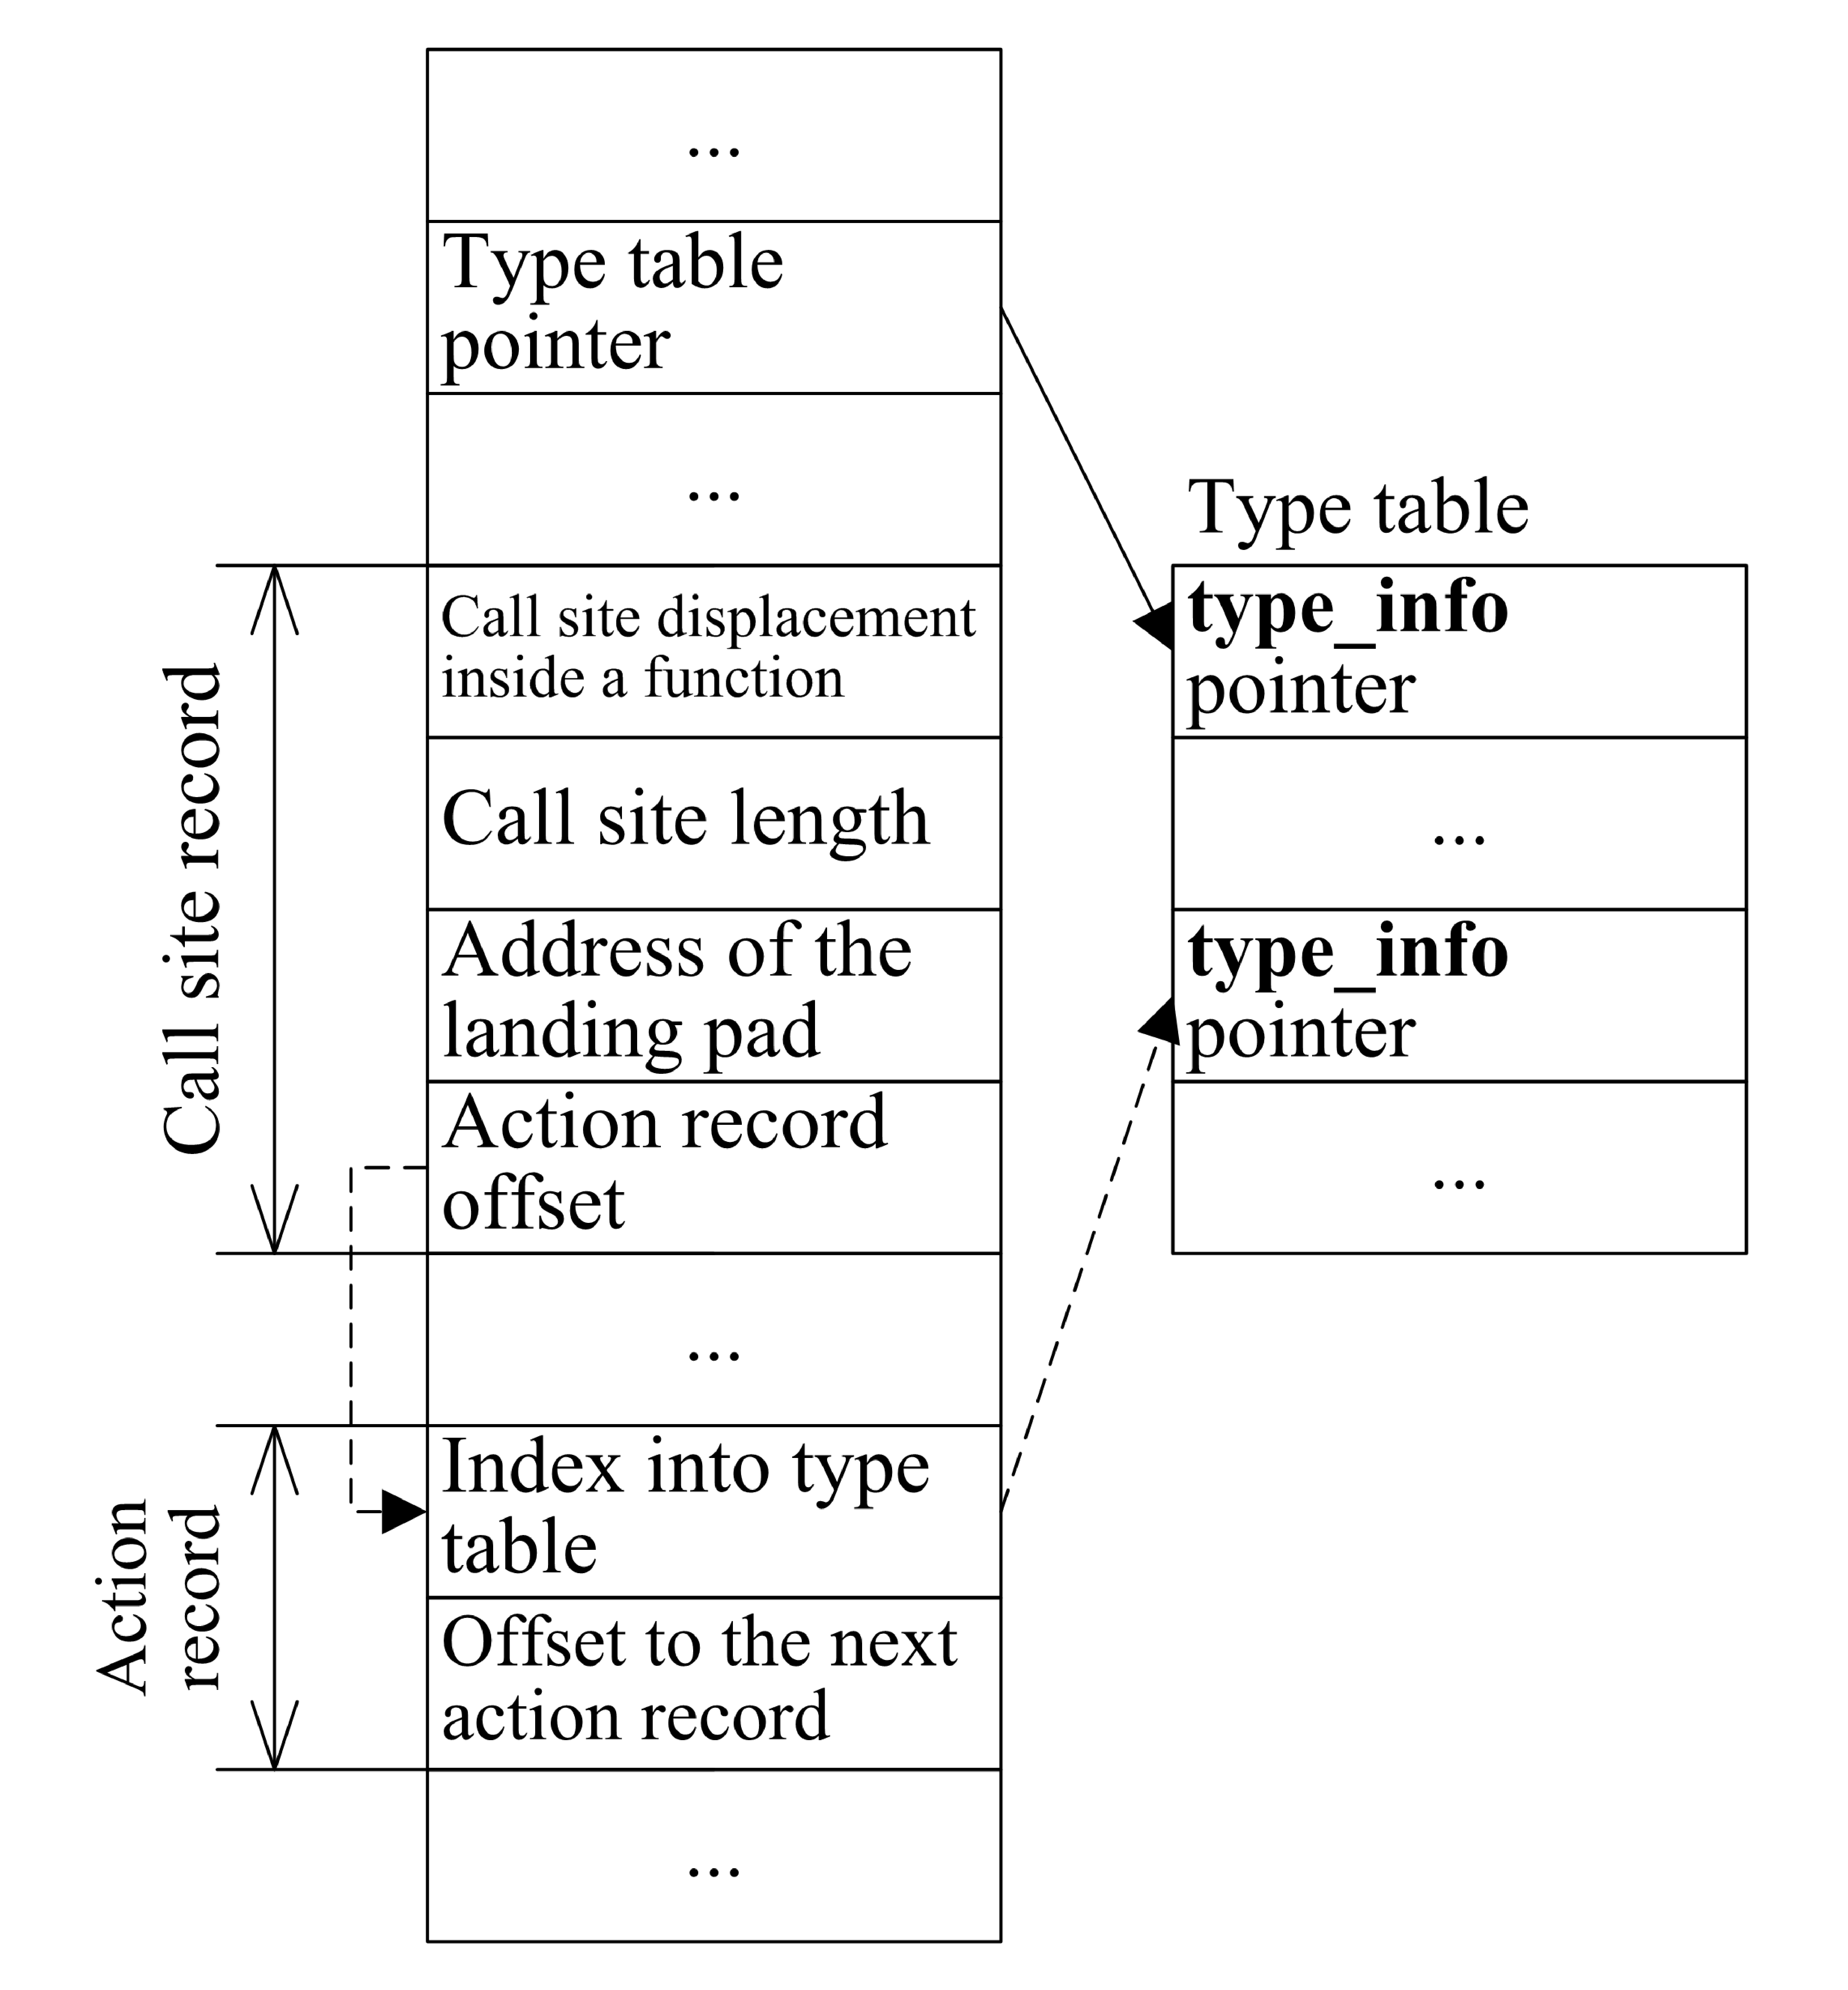
\includegraphics[width=8.0cm]{images/gcce}
%\vspace{-5mm}
\caption{Structures used by GCC for exception handling.}
\label{fig:gcce}
\end{figure}

For each call site a call site record is emitted by the compiler (see Fig. \ref{fig:gcce}). It contains:
\skipspace\begin{itemize}\compact
\item the call site displacement inside a function;
\item the call site length;
\item the address of the corresponding landing pad;
\item the pointer to the list of \textit{action records}.
\end{itemize}

Each action record contains an index of an element in the table 
of \lstinline{type_info} pointers.
The list of action records describes
exception types that are handled by the landing pad.

%Information stored in the statically allocated structures in
%\textbf{.eh\_frame} and \textbf{.gcc\_except\_table} sections must be
%parsed in order to reconstruct \lstinline{try} and \lstinline{catch}
%blocks.
%This presents no difficulties as the format of these structures
%is documented.

%Before the runtime transfers control to a landing pad, it 
%finds the index of exception's \lstinline{type_info}
%in the type table. This index is passed in \textbf{edx} register
%to the landing pad. Dispatch to the \lstinline{catch} block body is
%performed via a \lstinline{switch} on this index.

For quality reconstruction of exception handling, the following constructs must be recovered:
\skipspace\begin{itemize}\compact
\item catch blocks;
\item try blocks;
\item throw statements.
\end{itemize}

Each \lstinline{catch} block is referenced from its corresponding landing pad,
starts with a call to \lstinline{__cxa_begin_catch}
and ends with a call to \lstinline{__cxa_end_catch}.
Thus \lstinline{catch} blocks can be reconstructed by examining
the landing pad and the locations it references.

Different destructors must be called when exception is thrown from
different call sites. That's why the compiler generates several landing
pads for each \lstinline{try} block.
However, the part of the landing pad that performs dispatch to
the \lstinline{catch} block (the part on Fig.~\ref{fig:lpad}) is shared by all
landing pads for all call sites of a single \lstinline{try} block.

Therefore call sites belonging to the same \lstinline{try} block can be identified
by analyzing their corresponding landing pads~--- if two landing pads
share the same dispatch block, then their corresponding call sites
belong to the same \lstinline{try} block. Extents of the \lstinline{try}
block are then reconstructed by uniting the extents of all its corresponding
call sites.

Exception raising in GCC is performed via a call to the \lstinline{__cxa_throw} function:
{
\lstset{basicstyle=\footnotesize}
\begin{lstlisting}
void __cxa_throw(
  void *exception,
  type_info *typeInfo,
  void (*destructor)(void *)
);
\end{lstlisting}
}

To reconstruct throw statements it is sufficient to locate the calls
to \lstinline{__cxa_throw} and find the values of its parameters.

% TODO: explicit / implicit throw statements.
% I believe in C++ there are no implicit throws.


\section{Decompiler Architecture}\label{sectionArchitecture}\skipsectionspace
SmartDec decompiler is an experimental tool for analysis of programs
in assembly language and their transformation into high-level code
in C or C++ languages.
SmartDec's workflow follows the pipeline model. 
Decompilation comprises several phases each using results of one 
or more previous ones (see Fig.~\ref{fig:workflow}):

\skipspace\begin{enumerate}\compact
\item Parsing of the input assembly listing.
\item Building of the control flow graph. Isolation of functions.
\item Parsing of statically allocated exception handling structures and fixing of the control flow graph.
\item Transformation of assembly instructions into platform-independent program representation.
\item Reconstruction of classes and class hierarchies.
\item Analysis of functions:
\skipspace\begin{enumerate}\compact
  \item Joint reaching definitions and constant propagation analysis.
  \item Liveness analysis, dead code elimination.
  \item Reconstruction of local variables, function arguments and return values.
  \item Reconstruction of data types.
  \item Structural analysis.
\end{enumerate}
\item High-level program generation, optimization and output.
\end{enumerate}

\begin{figure}[tb!]
\centering
  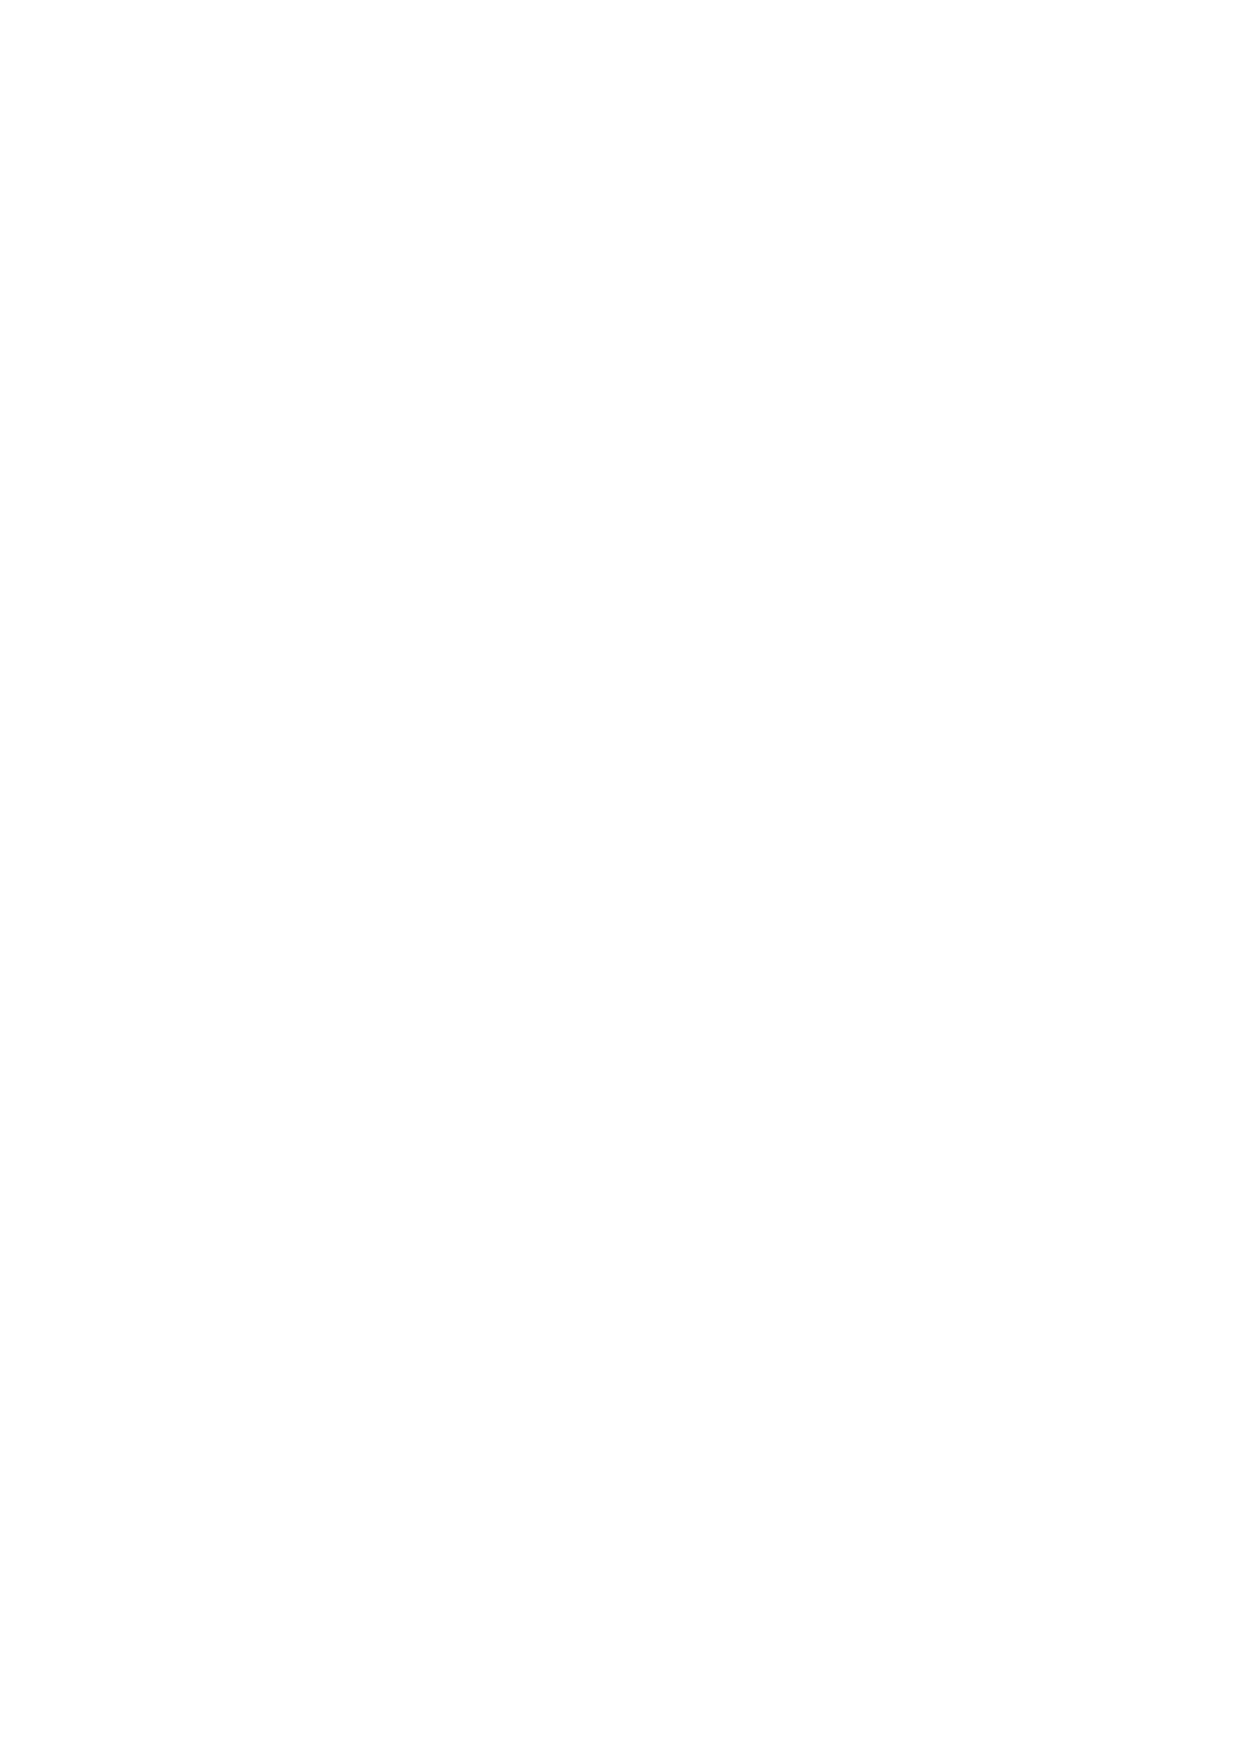
\includegraphics[width=8.0cm]{images/workflow}
%\vspace{-4mm}
\caption{Decompilation workflow.}
\label{fig:workflow}
\end{figure}

The rest of this section covers implementation details of some of these phases.

\subsection{Parsing}\skipsectionspace
Decompilation requires assembly listing of the program being analyzed to be supplied.
Generation of this listing is a task of a separate disassembler tool.

Currently SmartDec can parse the output of GNU \emph{objdump}
and Microsoft \emph{dumpbin} tools. 
SmartDec also integrates with IDA Pro Interactive Disassembler 
and can import information from its internal data structures.

At this phase the following objects are created:
\skipspace\begin{itemize}\compact
\item A sequence of instructions represented in a platform-dependent way.
\item An image object that contains information on the sections of the
  binary file and provides methods for reading its contents.
\end{itemize}


\subsection{Isolation of functions}\skipsectionspace
%Identification and isolation of functions is a required decompilation step. 
%Many subsequent analyses are performed on function level.
SmartDec uses a function reconstruction algorithm that is based on
the analysis of the program control flow graph.
In order to build this graph, instruction sequence is divided into
basic blocks. 
The following addresses are used as basic block boundaries:
\skipspace\begin{itemize}\compact
\item jump and call destinations;
\item addresses of instructions situated in memory immediately
after jump instructions and empty memory areas.
\end{itemize}
Edges between basic blocks are added according to the control flow
transfers performed by their last instructions.
Functions are then discovered as connected
components of undirected version of the control flow graph.

% TODO: can there be computed gotos?
% yegor: Why not? Nothing states the opposite. Only edges are not added for now.

\subsection{Intermediate representation}\skipsectionspace
Representation of a function as a control flow graph with
instructions inside basic blocks is not suitable for future
analyses that require knowledge about semantics of instructions.
Therefore, functions are translated into special intermediate
representation called Formulae.

In Formulae representation instruction semantics is expressed
in a sequence of \emph{statements}. 
Statement is a command for a virtual machine that can be used 
for partial simulation of input assembly program.

This virtual machine has its own memory model. 
The memory of this machine consists of independent address 
spaces identified by integer numbers. 
Each address space represents a block of linear memory with bit addressing. 
Such memory model allows to abstract away the actual locations 
of the tracked values. 
Registers, stack offsets and global addresses can be assigned 
their own memory locations from different address spaces 
and tracked uniformly.

Statements accept expressions as arguments.
These expressions are represented as expression trees.
Nodes of an expression tree will be further referred to as \emph{terms}.
Currently supported types of terms include integer
constant, memory location access (at a constant address),
dereference (of an expression), unary and binary arithmetic
operators.

The following types of statements are used:
\skipspace\begin{description}\compact
\item[Assignment] performs assignment of one expression to another (typically a memory location access or dereference).
\item[Kill] forgets about previous assignments to the given memory location.
\item[Jump] performs unconditional jump to the given address.
\item[Conditional jump] performs a jump to the given address when the given condition is true.
\item[Call] performs a function call to the given address.
\item[Return] returns from a function call.
\end{description}


\subsection{Dataflow analysis}\skipsectionspace
The goal of dataflow analysis is to construct the most complete set of reaching definitions for each term.
For this purpose joint reaching definition and constant propagation analysis \cite{muchnick97} is performed.
Such approach makes it possible to use already computed reaching definitions for further constant propagation and vice versa.
The joint analysis is finished upon reaching a fixed point.

% TODO: Нужно ли подробнее?

\subsection{Liveness analysis and dead code elimination}\skipsectionspace
The goal of liveness analysis is to find a set of terms that participate in 
calculations that are \textit{useful}. 
A calculation is considered \textit{useful} if its result can potentially 
affect program input, output or control flow. 
For example, calculation of a flag that is not used anywhere is not \textit{useful}.

Liveness analysis is performed by propagating the \textit{useful} state of each term
through the Formulae program representation. After liveness analysis is complete, all
the code that is not \textit{useful} can be safely eliminated. 
In our experience, dead code elimination for x86 programs reduces the number of 
terms in a program almost twofold, thus speeding up other analysis steps accordingly.


\subsection{Type reconstruction}\skipsectionspace

A set of attributes is associated with a type of each term.
Type reconstruction is done via deduction of these attributes,
which is performed iteratively until a fixed point is reached.
These attributes are then used directly for generation of
type declarations in a high-level language.

The following type attributes are used:
\skipspace\begin{description}\compact
\item[size] is the type size in bits;
\item[integer] is true if the type is an integer type;
\item[float] is true if the type is a float type;
\item[pointer] is true if the type is a pointer type;
\item[pointee] is a type of this type's dereference;
\item[signed] is true if the type is signed;
\item[unsigned] is true if the type is unsigned;
\item[factor] is a minimal value by which values of this type are
incremented or decremented. 
This attribute is used for reconstruction of arrays.
\item[offsets] is a mapping from integer offset to the type
of the field of this type at this offset.
This attribute is used for reconstruction of composite types.
\end{description}

Inference of the attributes that are used for basic type reconstruction
is performed according the rules described in \cite{wcre2008} and \cite{psi_workshop}.
Reconstruction of composite types is performed as it is described in \cite{scam2010}.

%For convenience, type attributes are organized in disjoint sets.
%Two type attributes are joined in the following cases:
%\skipspace\begin{itemize}\compact
%\item when they belong to terms accessing the same variable;
%\item when they are results of dereferencing the same pointer type;
%\item when they are the types of field access expressions of the 
%form $(base+offset)$ that have the same base type and offset.
%\end{itemize}
%Such organization improves the overall algorithm performance due to
%decreasing the number of required propagations and therefore
%the number of iterations until reaching a fixed point.


\subsection{Structural analysis}\skipsectionspace

In order to reconstruct high-level language control flow statements,
a variant \cite{PI3_09} of structural analysis \cite{muchnick97} is applied.

Structural analysis operates on control flow graphs of special kind.
Such graphs have \emph{regions} as nodes.
A region is a basic block or a subgraph with at most one \emph{entry} node.
The entry node of a region is a node that has incoming edges from outside
the region.

Region types include cyclic regions (generic loop, while, do-while),
conditionals (if-then, if-then-else, compound condition), block
regions and regions of unknown type. Initially, control flow graph
of a function contains single region comprising all basic blocks
of this function.
\begin{figure}[bt!]
\centering
%\vspace{-4mm}
  \includegraphics[height=4.0cm]{if-then-else.pdf}
%\vspace{-7mm}
\caption{Example of a pattern for if-then-else region.}
\label{fig:if-then-else}
\end{figure}

Structural analysis of a region is performed via pattern matching.
An example of a pattern for conditional statement is presented in Fig.~\ref{fig:if-then-else}. 
When a certain subgraph matches a pattern of
some region type, a new region of this type is created. 
All nodes of the subgraph under consideration are then moved into this region,
and all edges from (to) subgraph nodes are transformed into edges from (to) the region itself. 
Duplicate edges are then removed.

Compound conditions can be used in conditional loops and \lstinline{if} statements.
This is why they are reduced in the first place. 
This helps to correctly identify the type of the loop when it uses compound condition
and disallows reconstruction of compound conditions as series of enclosed \lstinline{if} statements.

Next, all cyclic regions are reduced. 
When a cyclic region is reduced, all edges corresponding to \lstinline{break}
and \lstinline{continue} statements are removed from it. This simplifies control
flow structure inside the loop and allows to recover conditional
statements with \lstinline{break} and \lstinline{continue} statements inside.
Since cyclic regions can have complex control flow structure inside,
structural analysis is performed in newly created cyclic regions recursively.

Then block statements are recovered in order to assemble each branch of
an \lstinline{if} statement into a single node.
At last, if-then and if-then-else regions are reduced.

The final fully reduced graph is used directly during code generation.
Control structure in generated program is conveyed via C control statements
and, when necessary, explicit control transfer operations \lstinline{break},
\lstinline{continue} and \lstinline{goto}. Computed gotos are represented
by \lstinline{goto} statements having expressions as the argument.

%\section{Code generation}
%
%Yep?



\section{Implementation and experimental results}\label{sectionExperiments}\skipsectionspace
% Available at \url{http://decompilation.info}.


\begin{figure}[tb!]
\centering
{
\lstset{basicstyle=\scriptsize}
\begin{lstlisting}
struct BinaryFunction {
  virtual int calculate(int a, int b) = 0;
};

struct GCD: public BinaryFunction {
  virtual int calculate(int a, int b);
};

struct Pow: public BinaryFunction {
  virtual int calculate(int a, int b);
};

int GCD::calculate(int a, int b) { 
  if (b == 0)
    return a;
  else
    return GCD::calculate(b, a % b);
}

int Pow::calculate(int a, int b) { 
  int result = 1;
  for(int i = 0; i < b; i++)
    result *= a;
  return result;
}
\end{lstlisting}
%\vspace{-6mm}
}
\caption{C++ source. Irrelevant code omitted.}
\label{fig:src_code}
\end{figure}

\begin{figure}[tb!]
\centering
{
\lstset{basicstyle=\scriptsize}
\begin{lstlisting}
struct C0 {
  virtual int32_t f_401367(int32_t a1, int32_t a2) = 0;
}

struct C1: C0 {
  virtual int32_t f_401367(int32_t a1, int32_t a2);
}

struct C2: C0 {
  virtual int32_t f_401367(int32_t a1, int32_t a2);
}

int32_t C1::f_401367(int32_t a1, int32_t a2) {
  if (a2 == 0) {
    return a1; 
  } else {
    return C1::f_401367(a2, a1 % a2);
  }
}

int32_t C2::f_401367(int32_t a1, int32_t a2) {
  int32_t v1;
  int32_t v2;
  v1 = 1;
  v2 = 0;
  while (v2 < a2) {
    v2 = v2 + 1;
    v1 = v1 * a1;
  }
  return v1;
}
\end{lstlisting}
%\vspace{-6mm}
}
\caption{Decompiled C++ source corresponding to the code on Fig.~\ref{fig:src_code}. Irrelevant code omitted.}
\label{fig:dec_code}
\end{figure}

SmartDec was tested on a variety of open-source software written in C++ and on
several hand-crafted tests. This section presents the results of testing
of C++-related functionality. The algorithms used for C decompilation do not undergo
significant changes when used for decompilation of C++ programs.
Experimental results of the basic type reconstruction algorithm that is used 
in SmartDec are presented in \cite{psi_workshop}.
Troshina et. al. presented an empirical study of the composite type reconstruction 
algorithm that is used in SmartDec \cite{scam2010}.
SmartDec's structural analysis algorithm has been analyzed in \cite{PI3_09}.

As SmartDec is yet unable to produce directly compilable code, 
the decompiled code cannot be tested by recompilation and has to be verified manually.
A fragment of one of the tests from our test suite is presented on Fig.~\ref{fig:src_code}. 
The corresponding decompiled code is presented on Fig.~\ref{fig:dec_code}.

%The description of the tests is presented in Table \ref{table:samples}.
%Column ``Name'' contains the name of the test program, column ``CLOC'' shows
%the number of C++ code lines, column ``ALOC'' shows the number of lines
%of assembly code and column ``Description'' contains the brief
%description of the test programs.

%\begin{table}[b!]
%\small
%\begin{tabular}{|l|l|l|l|}
%\hline
%Name       & CLOC   & ALOC & Description\\
%\hline
%lesDlgs    & 93     & 1086 & lesDlgs.cpp from Notepad++\\
%binFuncs   & 53     & 92   & Hand-crafted test\\
%\hline
%\end{tabular}
%\caption{Characteristics of the sample programs}
%\label{table:samples}
%\end{table}

%column ``CLOC'' shows
%the number of C++ code lines, column ``ALOC'' shows the number of lines
%of assembly code and column ``Description'' contains the brief
%description of the test programs.


Testing of the reconstruction of exception handling constructs was performed manually. 
Description of the tests is presented in Table \ref{table:samples}.
Columns ``Application'' and ``File'' contain the names of the application
and the source file of this application and columns ``Try'', ``Catch'' and ``Throw'' show 
the number of reconstructed \lstinline{try} blocks, \lstinline{catch} blocks and 
\lstinline{throw} statements respectively. 
Manual verification has shown that in all these tests all exception handling constructs 
present in source file were reconstructed correctly. No spurious constructs were recovered.

%and virtual function calls
%was performed manually. For testing we considered 

% TODO: rather small test suite

\begin{table}[b!]
\footnotesize
\begin{tabular}{|l|l|l|l|l|}
\hline
Application & File                 & Try   & Catch & Throw \\
\hline
notepad++   & Parameters.cpp       & 1     & 1     & 4     \\
shareaza    & Security.cpp         & 5     & 5     & 0     \\
shareaza    & DownloadGroups.cpp   & 3     & 3     & 0     \\
mongodb     & database.cpp         & 3     & 3     & 3     \\
---         & 061\_multi\_try.cpp  & 2     & 3     & 2     \\
\hline
\end{tabular}
%\vspace{-1mm}
\caption{Test results for exception reconstruction.}
\label{table:samples}
\end{table}

For testing of class hierarchy reconstruction correctness, the following automatic process is used.
First, the program is compiled with optimizations and RTTI enabled, and
RTTI-aware class hierarchy reconstruction algorithm is used to collect information
about polymorphic class hierarchy. This algorithm always provides correct results \cite{fokin10}.
The program is then recompiled with optimizations but without RTTI,
and class hierarchy reconstruction algorithm that does not use RTTI is applied.
Compiler-generated debug information is then used to restore the correspondence 
between class hierarchies reconstructed on the first and second steps. 
Two class hierarchies are then compared.

\begin{table}[b!]
\footnotesize
\begin{tabular}{| l | r | r | r | r |}
\hline
Application &          mysqld & shareaza & notepad++ & doxygen \\
\hline
Vtables found &         950   &   1128   &   95      & 415 \\
Non-vtables &           0.2\% &   0\%    &   0\%     & 0\% \\
Vtable mismatches &     3.1\% &    2.8\% & 4.0\%     & 4.8\% \\
Classes found &         918   &   1101   &  95       & 397 \\
Class mismatches &      5.5\% &    5.0\% & 10.5\%    & 6.3\% \\
\hline
\end{tabular}
%\vspace{-1mm}
\caption{Test results for class hierarchy reconstruction.}
\label{table:tests}
\end{table}

Test results are presented in Table~\ref{table:tests}.
For each of the analyzed applications all vtables present in
the assembly were found.

``Non-vtables'' row refers to the reconstructed vtables that were not present
in the source program. Static arrays of function pointers that are
used in the same way as vtables fall into this category.

Mismatch rates are calculated taking into account the following categories of classes.
\skipspace\begin{itemize}\compact
\item Classes that do not override any of the virtual functions of
    their bases. Vtables for such classes can be optimized away by
    the compiler, thus leading to incorrect class hierarchy reconstruction. 
	As this doesn't introduce any changes in the semantics of
    the program, such cases are not treated as mismatches.
\item Classes with no data members and no actions performed in
    constructors and destructors. Hierarchies of such classes can be
    rearranged in virtually any way without changing the semantics
    of the program. Such cases are not treated as mismatches.
\end{itemize}

``Vtable mismatches'' row refers to vtables where the reconstructed parent vtable
differs from the real one. For example, if a vtable was reconstructed
as not having a parent, while it actually has one, then this is a mismatch.
Most of vtable mismatches were registered as a result of the parent vtable
being located in a shared library. The reason for this is that SmartDec 
currently does not support joined analysis of several low-level programs.
Other mismatches were due to vtable pointer field 
initializations being optimized away by the compiler.

``Class mismatches'' row refers to classes where reconstructed vtables or parents
contradict to the real ones. Most of class mismatches fall into the
following two categories:
\skipspace\begin{itemize}\compact
\item Classes that contain mismatched vtables.
\item Classes that contain other polymorphic classes as fields.
    Inheritance and aggregation may be indistinguishable, 
	and this is why such mismatches do not necessarily 
	lead to misinterpretation of the program semantics.
\end{itemize}


\section{Conclusion and further work}\skipsectionspace
%We've shown that it's possible.

We have described the challenges of C++ decompilation and proposed
several methods that can be used to overcome them.
These methods allow automatic reconstruction
of polymorphic classes and hierarchies, 
virtual and non-virtual member functions, constructors and destructors,
calls to virtual functions,
types of class members and their layout,
types of variables that store pointers to polymorphic classes
and exception raising and handling statements.

Proposed methods were implemented in SmartDec, a C++ decompiler that is
being developed by the authors at Select LTD.
SmartDec was tested on a variety of open-source software written in C++
and showed good results.

Directions for future work include generation of C++ code that
can be compiled and tested without prior manual editing.

\bibliographystyle{IEEEtran}
\bibliography{wcre11}

\end{document}




















